\documentclass{standalone}
\usepackage{tikz}
\usepackage{tkz-fct}

\begin{document}

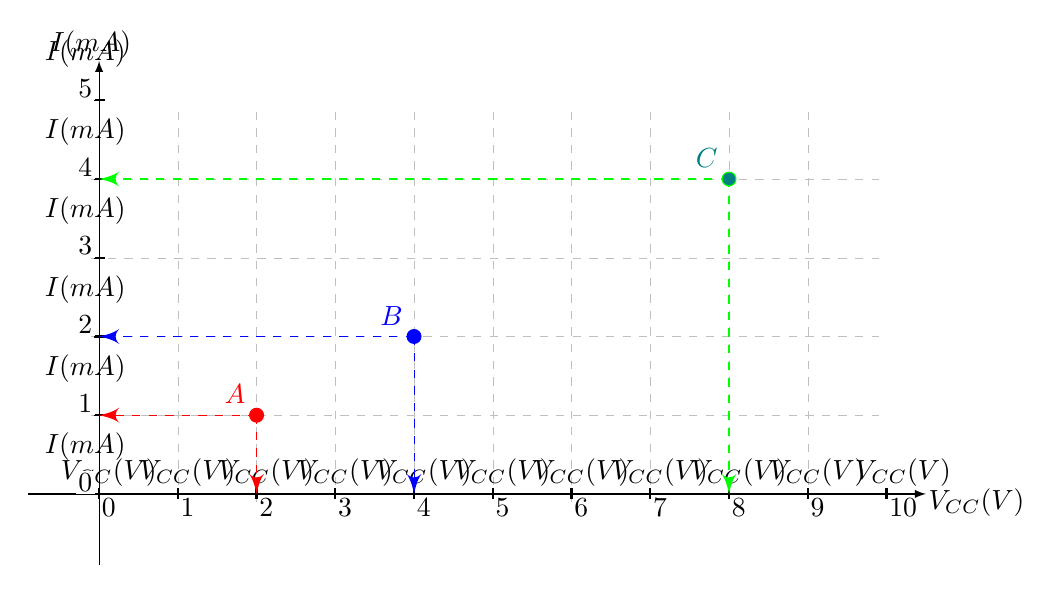
\begin{tikzpicture}[domain=0:10]
 		\tkzInit[xmin=-0.9,xmax=10,ymin=-0.9,ymax=5]
		\draw[ultra thin,dashed,color=lightgray] (-0.1,-0.1) grid (9.9,4.9);
		\tkzAxeX[label=$V_{CC}(V)$,right]
		\tkzAxeY[label=$I(mA)$,above]

 		\tkzFct[samples=2,line width=1.5pt, domain=0:10]{x/2}
		\tkzDefPointByFct[ref=A,with=a](2)
		\tkzDefPointByFct[ref=B,with=a](4)
		\tkzDefPointByFct[ref=C,with=a](8)
		\tkzPointShowCoord[color=red](A)
		\tkzPointShowCoord[color=blue](B)
		\tkzPointShowCoord[color=green](C)
		\tkzDrawPoint[color=red,fill=red,size=5](A){}
		\tkzText[above left,red](A){$A$}
		\tkzDrawPoint[color=blue,fill=blue,size=5](B){}
		\tkzText[above left,blue](B){$B$}
		\tkzDrawPoint[color=green,fill=teal,size=5](C){}
		\tkzText[above left,teal](C){$C$}

\end{tikzpicture}
\end{document}
